\documentclass{article}

%%% ---------------- %%%
%%% --- Packages --- %%%
%%% ---------------- %%%

\usepackage[utf8]{inputenc}
\usepackage{graphicx}       % for figure environment 
\usepackage{natbib}         % for citations
\usepackage[a4paper, left = 2.5cm, right = 2.5cm, top = 2.5cm, bottom = 2.5cm]{geometry}            % page layout
\usepackage{setspace}       % line spacing
\usepackage{mathptmx}       % Times new Roman 1
\usepackage[T1]{fontenc}    % Times new Roman 2
\usepackage{subcaption}     % subfigure environment
\usepackage{amsmath} 
\usepackage{caption} % For table caption
\usepackage{booktabs} % for prettier tables
\usepackage{placeins} % FloatBarrier command to force text between tables 
\usepackage{authblk} % For nice header with affiliation  
\usepackage{float}

\usepackage{caption} % The captionpackage allow for captions other than the normal numbers. Here, I need Table/ Figure S1 instead of just 1. 

%%% ---------------- %%%
%%% --- Settings --- %%%
%%% ---------------- %%%

\doublespacing      % double spaced
\pagestyle{empty}   % supress page numbering
% --- Title --- %

\title{
Should ecologists prefer model- over algorithm-based multivariate methods?\\
Supplementary Material
}
\author{}
\date{}

%%% ---------------- %%%
%%% --- Document --- %%%
%%% ---------------- %%%

\begin{document}

\maketitle


\section{Calculating pseudo \textit{p}-values for CQO} 
    Currently, the VGAM R-package \citep[Version 1.1-1,][]{VGAM19} does not implement hypothesis tests regarding the predictors in a CQO. 
    % 
    As we relied on \textit{p}-values to compare the tested methods, we calculated pseudo \textit{p}-values for CQO using a permutation-based test. 
    % 
    We used the absolute sum of constrained coefficients ($ C_{\sum} $) as the test statistic.
    % 
    The constrained coefficient $C_{ij}$ is the weight of the variable $X_i$ on the latent variable $\nu_j$, the higher $C_{ij}$ is the stronger $X_i$ influences $\nu_j$. 
    % 
    By summing $C_{i}$ over all latent variables, we test the impact that $X_i$ has on the model as a whole. 
    % 
    In this summation, we used the absolute values and removed the mathematical sign as these only signify the direction of influence, not its magnitude. 
    % 
    We do not know what distribution to expect from this statistic or if it adheres to a specific distribution. 
    % 
    The method of choice for such cases are permutation-based tests, which produce pseudo \textit{p}-values \citep{legendre2012numerical}. 
    %
    Their general approach is as follows: 
    % 
    A test statistic $T$ is computed for the data set of interest $D$, with $X,Y \in D$. 
    % 
    Some property of $D$ (e.g. the rows of $X$ or $Y$) is permuted $n$-times and the same test statistic is calculated for each of the permuted data sets $D^*$. 
    % 
    The pseudo-\textit{p}-value can then be calculated as: 
    % 
    \begin{center} 
    $p = \displaystyle \dfrac{\sum_{j=1}^n(k_j)}{n + 1}$ \hspace{1cm} 
    with 
    \hspace{1cm} $k_j = \begin{cases} 1 &\text{if\ $T^*_j \ge T$} \\ 0 & \text{else} \end{cases}$\\ 
    \end{center}

    %
    We permuted the predictors. 
    % 
    Each predictor was tested separately so that in any one model only one predictor was permuted while the other remained in their original order. 
    \newpage
\section{Supplementary figures and tables}   
% \section{Simulation parameters} 
%     Table \ref{tab:SimDet} shows the model parameters used in the simulations. The optimum parameter \textit{u} is the only instance of a parameter that is relevant to both gradients and differs between them. 
% 		%
% 		The different values are separated by forward slashes. 
% 		%
% 		Bimodal gradients require two optima per species. 
% 		%
% 		The used combinations are shown in square brackets. \\
		
		% ------------------------- %
		%& Table: Model parameters 
		% ------------------------- %
		% function from the caption package 
	\captionsetup[table]{name=Table S}
	\begin{table}[!htbp] 
		\centering 
        \caption{
            Model parameters used in simulations. An x indicates that the parameter is not relevant to the respective gradient type. \textit{c} is the maximal abundance, \textit{t} the tolerance, \textit{u} the location of the optimum and $\beta$ the  linear response parameter. Values in square brackets are the pairs of optima for bimodal gradients.
        }
        \label{tab:mvglm:ss} 
        \begin{tabular}{@{\extracolsep{5pt}} cccll}
			\\[-1.8ex]\hline 
            \hline \\[-1.8ex] 
            % Table body 
                %Header 
			    & \textit{c} & \textit{t} & \textit{u} &\ $beta$ \\
			\hline \\[-1.8ex]
				% Row 1 
				\textit{UU} & 100 & 7.5 & 20, 50, 80  & x                 \\
				% Row 2
				\textit{UL} & 100 & 7.5 & 10, 20, 30, 40, 50,60,70,80,90 &  0.1  \\
				% Row 3
				\textit{UB} & 100 & 5   & 20, 50, 80,  [10, 30 ],  [40, 60 ],  [70, 90 ]  & x \\
				% Row 4
				\textit{LL}   & x   & x   & x & 0.1, 0.2125, 0.3250, 0.4375, 0.5500, \\
				&&&& 0.6625, 0.7750, 0.8875, 1.0000 &      \\ 
				% Row 5
			    \textit{LB}  & 100 & 6   & [5, 25], [25, 45], [35, 55], [55, 75], [75, 95] & 0.1   \\
			    % Row 6
				\textit{BB}   & 100 & 6   & [5, 25], [35, 55], [75, 95] & x  \\
			\hline \\[-1.8ex] 
	    \end{tabular}
		\label{tab:SimDet}
	\end{table}
% page break 		
	\newpage
    % function from the caption package 
    \captionsetup[figure]{name=Figure S}
    \begin{figure}[!htbp]
        \centering
        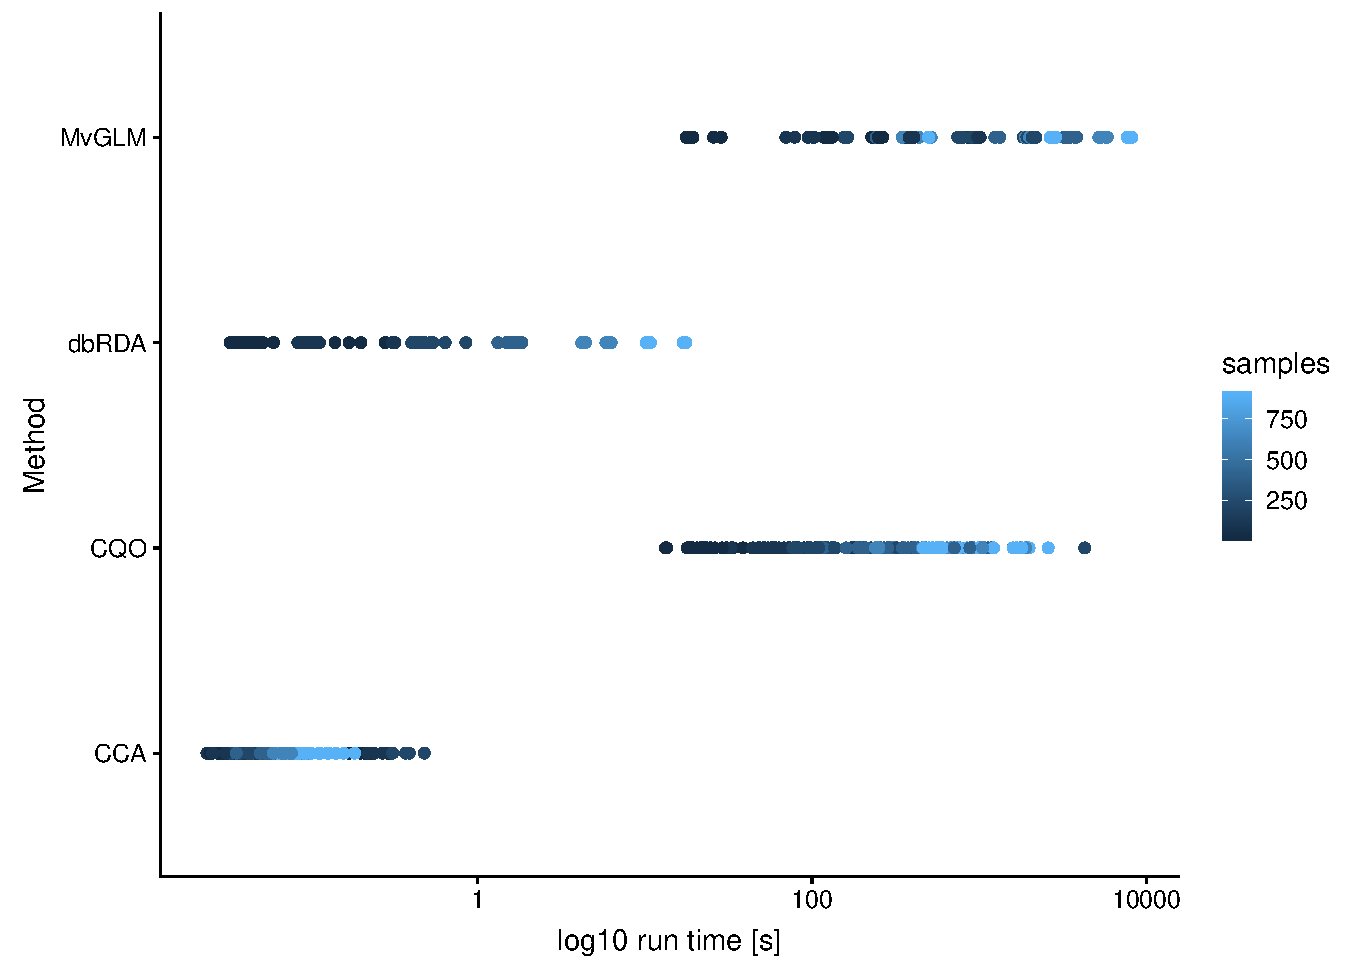
\includegraphics[scale = 0.4]{figures/runtimeplot.pdf}
        \caption{The Dunn-Smyth residuals of the \textit{LL} community sampled with 400 samples plotted against the linear predictor. A pronounced arched pattern can be observed for each single species (different colors).}
        \label{fig:arched_DS}
    \end{figure}{}
    
 % page break 		
	\newpage   
    
    \begin{figure}[!htbp]
        \centering
        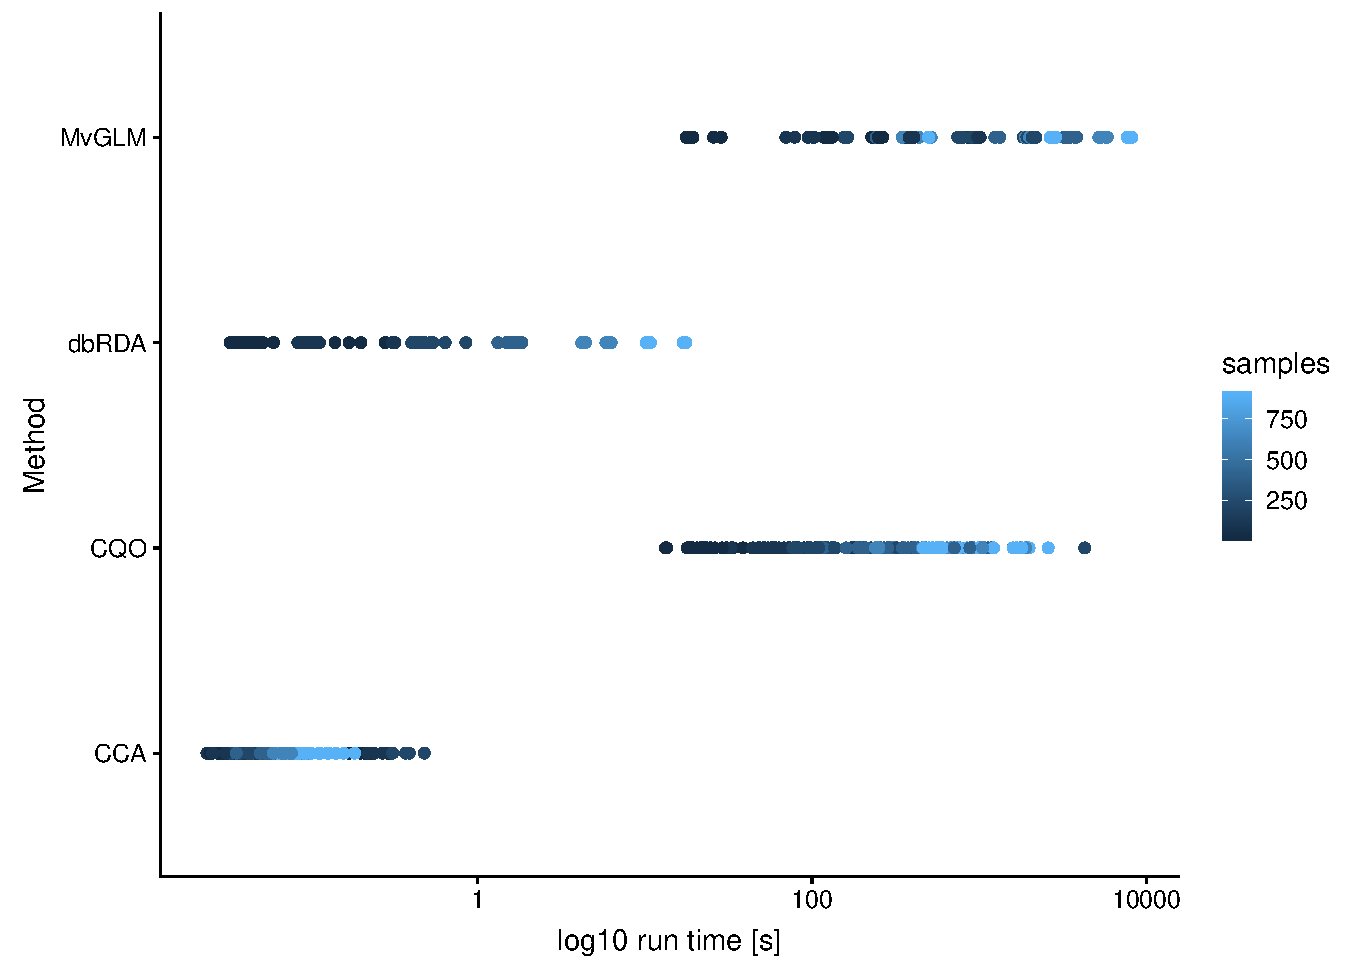
\includegraphics[scale =0.6]{figures/runtimeplot.pdf}
        \caption{Run times of Multivariate Generalized Linear Models (MvGLM), distance-based Redundancy Analysis (dbRDA), Constrained Quadratic Ordination (CQO), and Canonical Correspondence Analysis (CCA). X-axis is scaled with a decimal logarithm. Colors indicate sample sizes.}
        \label{fig:runtime}
    \end{figure}{}

% 	Mean run time of CCA was below one second (s) and that of dbRDA was 4.3 s. 
% 	%
% 	There were no significant differences between different response types or sample sizes. 
% 	%
% 	CQO was the faster model-based method with a mean run time of 365 s.
% 	%
% 	Between response types, speed differed from 175 s (\textit{LL}) to 592 s (\textit{UB}). 
% 	%
% 	Mean run time increased linearly with sample size form 27 s (n = 25) to  972 s (n = 900).
% 	%
% 	MvGLM was the slowest method with a mean run time of 2159 s.
% 	%
% 	Again speed differed between response types and again \textit{LL} was the fastest with  741 s while \textit{BB} was the slowest with a mean run time of 3337 s.
% 	%
% 	Here too, run time increased linearly with samples size form 174 s (n = 25) to 5055 s (n = 900).
% 	%
% 	Note, however, that the times for CQO do not include the calculation of p-values which is quite time-consuming. 
% \section{Further Result Statistics}	

% page break 		
	\newpage	
% 		This section contains all the mean \textit{p}-values at the level of response types or sample sizes.\\
% 		%
% 		Tables \ref{tab:mvglm:ss} and \ref{tab:mvglm:rs} show the mean \textit{p}-values of MvGLMs. 
% 		%
% 		% ------------------------------------------ %
% 		%& TABLE: GLM multivariate p-Value of Classes
% 		% ------------------------------------------- %
\begin{table}[!htbp] 
    \centering 
    \caption{
    Mean \textit{p}-values of Multivariate Generalized Linear Models with standard deviations for combinations of sample size and response type.
    } 
  \label{} 
    \begin{tabular}{@{\extracolsep{5pt}} cccccccc} 
    \\[-1.8ex]\hline 
    \hline \\[-1.8ex] 
    && \multicolumn{2}{c}{env1} & \multicolumn{2}{c}{env2} & \multicolumn{2}{c}{Noise}\\\cmidrule(l){3-4} \cmidrule(l){5-6} \cmidrule(l){7-8}
    %
    && $\mu$ & $\sigma$ & $\mu$ & $\sigma$ & $\mu$ & $\sigma$\\ 
    \hline \\[-1.8ex] 
    UU & $25$ & $0.002$ & $0.001$ & $0.016$ & $0.005$ & $0.342$ & $0.228$ \\ 
    UU & $100$ & $0.001$ & $0$ & $0.001$ & $0$ & $0.612$ & $0.267$ \\ 
    UU & $225$ & $0.001$ & $0$ & $0.001$ & $0$ & $0.697$ & $0.265$ \\ 
    UU & $400$ & $0.001$ & $0$ & $0.001$ & $0$ & $0.849$ & $0.129$ \\ 
    UU & $625$ & $0.001$ & $0$ & $0.001$ & $0$ & $0.875$ & $0.138$ \\ 
    UU & $900$ & $0.001$ & $0$ & $0.001$ & $0$ & $0.801$ & $0.219$ \\ 
    UL & $25$ & $0.001$ & $0$ & $0.146$ & $0.007$ & $0.781$ & $0.162$ \\ 
    UL & $100$ & $0.001$ & $0$ & $0.001$ & $0$ & $0.738$ & $0.210$ \\ 
    UL & $225$ & $0.001$ & $0$ & $0.001$ & $0$ & $0.727$ & $0.283$ \\ 
    UL & $400$ & $0.001$ & $0$ & $0.001$ & $0$ & $0.729$ & $0.258$ \\ 
    UL & $625$ & $0.001$ & $0$ & $0.001$ & $0$ & $0.642$ & $0.250$ \\ 
    UL & $900$ & $0.001$ & $0$ & $0.001$ & $0$ & $0.645$ & $0.272$ \\ 
    UB & $25$ & $0.022$ & $0.003$ & $0.125$ & $0.010$ & $0.477$ & $0.256$ \\ 
    UB & $100$ & $0.001$ & $0$ & $0.001$ & $0$ & $0.596$ & $0.264$ \\ 
    UB & $225$ & $0.001$ & $0$ & $0.001$ & $0$ & $0.737$ & $0.224$ \\ 
    UB & $400$ & $0.001$ & $0$ & $0.001$ & $0$ & $0.788$ & $0.171$ \\ 
    UB & $625$ & $0.001$ & $0$ & $0.001$ & $0$ & $0.784$ & $0.249$ \\ 
    UB & $900$ & $0.001$ & $0$ & $0.001$ & $0$ & $0.811$ & $0.170$ \\ 
    LL & $25$ & $0.001$ & $0.0004$ & $0.001$ & $0$ & $0.406$ & $0.192$ \\ 
    LL & $100$ & $0.001$ & $0$ & $0.001$ & $0$ & $0.587$ & $0.277$ \\ 
    LL & $225$ & $0.001$ & $0$ & $0.001$ & $0$ & $0.514$ & $0.301$ \\ 
    LL & $400$ & $0.001$ & $0$ & $0.001$ & $0$ & $0.574$ & $0.338$ \\ 
    LL & $625$ & $0.001$ & $0$ & $0.001$ & $0$ & $0.593$ & $0.319$ \\ 
    LL & $900$ & $0.001$ & $0$ & $0.001$ & $0$ & $0.460$ & $0.301$ \\ 
    LB & $25$ & $0.166$ & $0.010$ & $0.001$ & $0$ & $0.776$ & $0.162$ \\ 
    LB & $100$ & $0.001$ & $0$ & $0.001$ & $0$ & $0.717$ & $0.222$ \\ 
    LB & $225$ & $0.001$ & $0$ & $0.001$ & $0$ & $0.736$ & $0.285$ \\ 
    LB & $400$ & $0.001$ & $0$ & $0.001$ & $0$ & $0.721$ & $0.257$ \\ 
    LB & $625$ & $0.001$ & $0$ & $0.001$ & $0$ & $0.639$ & $0.269$ \\ 
    LB & $900$ & $0.001$ & $0$ & $0.001$ & $0$ & $0.643$ & $0.275$ \\ 
    BB & $25$ & $0.001$ & $0$ & $0.010$ & $0.002$ & $0.363$ & $0.242$ \\ 
    BB & $100$ & $0.001$ & $0$ & $0.001$ & $0$ & $0.432$ & $0.230$ \\ 
    BB & $225$ & $0.001$ & $0$ & $0.001$ & $0$ & $0.618$ & $0.276$ \\ 
    BB & $400$ & $0.001$ & $0$ & $0.001$ & $0$ & $0.828$ & $0.158$ \\ 
    BB & $625$ & $0.001$ & $0$ & $0.001$ & $0$ & $0.814$ & $0.191$ \\ 
    BB & $900$ & $0.001$ & $0$ & $0.001$ & $0$ & $0.717$ & $0.222$ \\ 
    \hline \\[-1.8ex] 
    \end{tabular} 
    \end{table} 

% page break 		
	\newpage	
	
	 %% -- CQO -- %% 
	 
	\begin{table}[!htbp] \centering 
        \caption{
            Mean \textit{p}-values of Constrained Quadratic Ordination with standard deviations for combinations of sample size and response type.
        } 
        \label{} 
        \begin{tabular}{@{\extracolsep{5pt}} cccccccc} 
            \\[-1.8ex]\hline 
            \hline \\[-1.8ex] 
            && \multicolumn{2}{c}{env1} & \multicolumn{2}{c}{env2} & \multicolumn{2}{c}{Noise}\\\cmidrule(l){3-4} \cmidrule(l){5-6} \cmidrule(l){7-8}
            %
            && $\mu$ & $\sigma$ & $\mu$ & $\sigma$ & $\mu$ & $\sigma$\\ 
            \hline \\[-1.8ex] 
            UU & $25$ & $0$ & $0$ & $0$ & $0$ & $0.820$ & $0.105$ \\ 
            UU & $100$ & $0$ & $0$ & $0$ & $0$ & $0.879$ & $0.082$ \\ 
            UU & $225$ & $0$ & $0$ & $0$ & $0$ & $0.875$ & $0.126$ \\ 
            UU & $400$ & $0$ & $0$ & $0$ & $0$ & $0.917$ & $0.052$ \\ 
            UU & $625$ & $0$ & $0$ & $0$ & $0$ & $0.880$ & $0.134$ \\ 
            UU & $900$ & $0$ & $0$ & $0$ & $0$ & $0.952$ & $0.050$ \\ 
            UL & $25$ & $0.127$ & $0.158$ & $0.289$ & $0.183$ & $0.646$ & $0.146$ \\ 
            UL & $100$ & $0.071$ & $0.098$ & $0.240$ & $0.258$ & $0.612$ & $0.267$ \\ 
            UL & $225$ & $0.004$ & $0.005$ & $0.010$ & $0.012$ & $0.506$ & $0.298$ \\ 
            UL & $400$ & $0.006$ & $0.013$ & $0.087$ & $0.168$ & $0.569$ & $0.196$ \\ 
            UL & $625$ & $0$ & $0$ & $0.519$ & $0.269$ & $0.990$ & $0$ \\ 
            UL & $900$ & $0.008$ & $0.018$ & $0.705$ & $0.401$ & $0.990$ & $0$ \\ 
            UB & $100$ & $0.024$ & $0.023$ & $0.026$ & $0.026$ & $0.654$ & $0.270$ \\ 
            UB & $225$ & $0.026$ & $0.058$ & $0.014$ & $0.031$ & $0.702$ & $0.206$ \\ 
            UB & $400$ & $0.036$ & $0.060$ & $0.002$ & $0.004$ & $0.658$ & $0.274$ \\ 
            UB & $625$ & $0.010$ & $0.022$ & $0.020$ & $0.044$ & $0.583$ & $0.385$ \\ 
            UB & $900$ & $0$ & $0$ & $0$ & $0$ & $0.639$ & $0.337$ \\ 
            LL & $25$ & $0.085$ & $0.048$ & $0.143$ & $0.090$ & $0.400$ & $0.183$ \\ 
            LL & $100$ & $0.154$ & $0.117$ & $0.095$ & $0.062$ & $0.723$ & $0.176$ \\ 
            LL & $225$ & $0.091$ & $0.075$ & $0.081$ & $0.060$ & $0.841$ & $0.102$ \\ 
            LL & $400$ & $0.180$ & $0.137$ & $0.263$ & $0.227$ & $0.761$ & $0.191$ \\ 
            LL & $625$ & $0.281$ & $0.201$ & $0.208$ & $0.191$ & $0.779$ & $0.126$ \\ 
            LL & $900$ & $0.295$ & $0.099$ & $0.188$ & $0.146$ & $0.838$ & $0.116$ \\ 
            LB & $25$ & $0.265$ & $0.127$ & $0.141$ & $0.159$ & $0.619$ & $0.158$ \\ 
            LB & $100$ & $0.097$ & $0.090$ & $0.038$ & $0.058$ & $0.619$ & $0.278$ \\ 
            LB & $225$ & $0.067$ & $0.109$ & $0.006$ & $0.013$ & $0.589$ & $0.272$ \\ 
            LB & $400$ & $0.174$ & $0.237$ & $0.006$ & $0.009$ & $0.586$ & $0.240$ \\ 
            LB & $625$ & $0.204$ & $0.166$ & $0.044$ & $0.061$ & $0.504$ & $0.260$ \\ 
            LB & $900$ & $0.164$ & $0.314$ & $0.020$ & $0.028$ & $0.561$ & $0.218$ \\ 
            BB & $25$ & $0$ & $0$ & $0$ & $0$ & $0.591$ & $0.233$ \\ 
            BB & $100$ & $0$ & $0$ & $0$ & $0$ & $0.359$ & $0.272$ \\ 
            BB & $225$ & $0$ & $0$ & $0$ & $0$ & $0.573$ & $0.299$ \\ 
            BB & $400$ & $0$ & $0$ & $0$ & $0$ & $0.636$ & $0.317$ \\ 
            BB & $625$ & $0$ & $0$ & $0$ & $0$ & $0.421$ & $0.271$ \\ 
            BB & $900$ & $0$ & $0$ & $0$ & $0$ & $0.543$ & $0.353$ \\ 
            \hline \\[-1.8ex] 
        \end{tabular} 
    \end{table}
	
% page break 		
	\newpage		
	
    %% -- CCA -- %% 
    \begin{table}[!htbp] \centering 
        \caption{
            Mean \textit{p}-values of Canonical Correspondence Analysis with standard deviations for combinations of sample size and response type.
        } 
        \label{} 
        \begin{tabular}{@{\extracolsep{5pt}} cccccccc} 
            \\[-1.8ex]\hline 
            \hline \\[-1.8ex] 
            && \multicolumn{2}{c}{env1} & \multicolumn{2}{c}{env2} & \multicolumn{2}{c}{Noise}\\\cmidrule(l){3-4} \cmidrule(l){5-6} \cmidrule(l){7-8}
            %
            && $\mu$ & $\sigma$ & $\mu$ & $\sigma$ & $\mu$ & $\sigma$\\ 
            \hline \\[-1.8ex] 
            UU & $25$ & $0.001$ & $0$ & $0.001$ & $0$ & $0.001$ & $0$ \\ 
            UU & $100$ & $0.001$ & $0$ & $0.001$ & $0$ & $0.467$ & $0.355$ \\ 
            UU & $225$ & $0.001$ & $0$ & $0.001$ & $0$ & $0.093$ & $0.113$ \\ 
            UU & $400$ & $0.001$ & $0$ & $0.001$ & $0$ & $0.349$ & $0.336$ \\ 
            UU & $625$ & $0.001$ & $0$ & $0.001$ & $0$ & $0.153$ & $0.275$ \\ 
            UU & $900$ & $0.001$ & $0$ & $0.001$ & $0$ & $0.247$ & $0.362$ \\ 
            UL & $25$ & $0.001$ & $0$ & $0.987$ & $0.014$ & $0.403$ & $0.288$ \\ 
            UL & $100$ & $0.001$ & $0$ & $1$ & $0$ & $0.329$ & $0.294$ \\ 
            UL & $225$ & $0.001$ & $0$ & $1$ & $0$ & $0.346$ & $0.274$ \\ 
            UL & $400$ & $0.001$ & $0$ & $1$ & $0$ & $0.393$ & $0.317$ \\ 
            UL & $625$ & $0.001$ & $0$ & $1$ & $0$ & $0.436$ & $0.219$ \\ 
            UL & $900$ & $0.001$ & $0$ & $1$ & $0$ & $0.439$ & $0.321$ \\ 
            UB & $25$ & $0.001$ & $0$ & $0.001$ & $0$ & $0.035$ & $0.074$ \\ 
            UB & $100$ & $0.001$ & $0$ & $0.001$ & $0$ & $0.344$ & $0.269$ \\ 
            UB & $225$ & $0.001$ & $0$ & $0.001$ & $0$ & $0.244$ & $0.283$ \\ 
            UB & $400$ & $0.001$ & $0$ & $0.001$ & $0$ & $0.172$ & $0.195$ \\ 
            UB & $625$ & $0.001$ & $0$ & $0.001$ & $0$ & $0.111$ & $0.192$ \\ 
            UB & $900$ & $0.001$ & $0$ & $0.001$ & $0$ & $0.066$ & $0.170$ \\ 
            LL & $25$ & $0.992$ & $0.012$ & $0.997$ & $0.005$ & $0.976$ & $0.031$ \\ 
            LL & $100$ & $0.985$ & $0.009$ & $0.989$ & $0.005$ & $0.994$ & $0.011$ \\ 
            LL & $225$ & $0.712$ & $0.046$ & $0.691$ & $0.031$ & $0.962$ & $0.069$ \\ 
            LB & $25$ & $0.987$ & $0.015$ & $0.001$ & $0$ & $0.398$ & $0.289$ \\ 
            LB & $100$ & $1$ & $0$ & $0.001$ & $0$ & $0.358$ & $0.307$ \\ 
            LB & $225$ & $1$ & $0$ & $0.001$ & $0$ & $0.378$ & $0.278$ \\ 
            LB & $400$ & $1$ & $0$ & $0.001$ & $0$ & $0.412$ & $0.331$ \\ 
            LB & $625$ & $1$ & $0$ & $0.001$ & $0$ & $0.438$ & $0.209$ \\ 
            LB & $900$ & $1$ & $0$ & $0.001$ & $0$ & $0.446$ & $0.321$ \\ 
            BB & $25$ & $0.001$ & $0$ & $0.001$ & $0$ & $0.564$ & $0.286$ \\ 
            BB & $100$ & $0.001$ & $0$ & $0.001$ & $0$ & $0.469$ & $0.341$ \\ 
            BB & $225$ & $0.001$ & $0$ & $0.001$ & $0$ & $0.580$ & $0.301$ \\ 
            BB & $400$ & $0.001$ & $0$ & $0.001$ & $0$ & $0.566$ & $0.314$ \\ 
            BB & $625$ & $0.001$ & $0$ & $0.001$ & $0$ & $0.497$ & $0.343$ \\ 
            BB & $900$ & $0.001$ & $0$ & $0.001$ & $0$ & $0.491$ & $0.330$ \\ 
            \hline \\[-1.8ex] 
        \end{tabular} 
    \end{table}
% page break 		
	\newpage		
	
    %% -- dbRDA -- %% 
    \begin{table}[!htbp] \centering 
        \caption{
            Mean \textit{p}-values of distance-based Redundancy Analysis with standard deviations for combinations of sample size and response type.
        } 
        \label{} 
        \begin{tabular}{@{\extracolsep{5pt}} cccccccc} 
            \\[-1.8ex]\hline 
            \hline \\[-1.8ex] 
            && \multicolumn{2}{c}{env1} & \multicolumn{2}{c}{env2} & \multicolumn{2}{c}{Noise}\\\cmidrule(l){3-4} \cmidrule(l){5-6} \cmidrule(l){7-8}
            %
            && $\mu$ & $\sigma$ & $\mu$ & $\sigma$ & $\mu$ & $\sigma$\\ 
            \hline \\[-1.8ex] 
            UU & $25$ & $0.001$ & $0$ & $0.001$ & $0$ & $0.510$ & $0.302$ \\ 
            UU & $100$ & $0.001$ & $0$ & $0.001$ & $0$ & $0.669$ & $0.304$ \\ 
            UU & $225$ & $0.001$ & $0$ & $0.001$ & $0$ & $0.457$ & $0.238$ \\ 
            UU & $400$ & $0.001$ & $0$ & $0.001$ & $0$ & $0.611$ & $0.275$ \\ 
            UU & $625$ & $0.001$ & $0$ & $0.001$ & $0$ & $0.561$ & $0.173$ \\ 
            UU & $900$ & $0.001$ & $0$ & $0.001$ & $0$ & $0.451$ & $0.275$ \\ 
            UL & $25$ & $0.001$ & $0$ & $0.066$ & $0.010$ & $0.553$ & $0.240$ \\ 
            UL & $100$ & $0.001$ & $0$ & $0.001$ & $0$ & $0.517$ & $0.275$ \\ 
            UL & $225$ & $0.001$ & $0$ & $0.001$ & $0$ & $0.470$ & $0.268$ \\ 
            UL & $400$ & $0.001$ & $0$ & $0.001$ & $0$ & $0.581$ & $0.278$ \\ 
            UL & $625$ & $0.001$ & $0$ & $0.001$ & $0$ & $0.529$ & $0.199$ \\ 
            UL & $900$ & $0.001$ & $0$ & $0.001$ & $0$ & $0.437$ & $0.228$ \\ 
            UB & $25$ & $0.001$ & $0$ & $0.001$ & $0$ & $0.486$ & $0.291$ \\ 
            UB & $100$ & $0.001$ & $0$ & $0.001$ & $0$ & $0.712$ & $0.245$ \\ 
            UB & $225$ & $0.001$ & $0$ & $0.001$ & $0$ & $0.435$ & $0.235$ \\ 
            UB & $400$ & $0.001$ & $0$ & $0.001$ & $0$ & $0.629$ & $0.234$ \\ 
            UB & $625$ & $0.001$ & $0$ & $0.001$ & $0$ & $0.591$ & $0.119$ \\ 
            UB & $900$ & $0.001$ & $0$ & $0.001$ & $0$ & $0.424$ & $0.272$ \\ 
            LL & $25$ & $0.010$ & $0.005$ & $0.009$ & $0.007$ & $0.520$ & $0.219$ \\ 
            LL & $100$ & $0.001$ & $0$ & $0.001$ & $0$ & $0.467$ & $0.261$ \\ 
            LL & $225$ & $0.001$ & $0$ & $0.001$ & $0$ & $0.477$ & $0.261$ \\ 
            LL & $400$ & $0.001$ & $0$ & $0.001$ & $0$ & $0.665$ & $0.293$ \\ 
            LL & $625$ & $0.001$ & $0$ & $0.001$ & $0$ & $0.589$ & $0.290$ \\ 
            LL & $900$ & $0.001$ & $0$ & $0.001$ & $0$ & $0.347$ & $0.298$ \\ 
            LB & $25$ & $0.044$ & $0.008$ & $0.001$ & $0$ & $0.550$ & $0.241$ \\ 
            LB & $100$ & $0.001$ & $0$ & $0.001$ & $0$ & $0.514$ & $0.277$ \\ 
            LB & $225$ & $0.001$ & $0$ & $0.001$ & $0$ & $0.473$ & $0.266$ \\ 
            LB & $400$ & $0.001$ & $0$ & $0.001$ & $0$ & $0.584$ & $0.276$ \\ 
            LB & $625$ & $0.001$ & $0$ & $0.001$ & $0$ & $0.521$ & $0.194$ \\ 
            LB & $900$ & $0.001$ & $0$ & $0.001$ & $0$ & $0.437$ & $0.224$ \\ 
            BB & $25$ & $0.001$ & $0$ & $0.001$ & $0$ & $0.564$ & $0.296$ \\ 
            BB & $100$ & $0.001$ & $0$ & $0.001$ & $0$ & $0.572$ & $0.316$ \\ 
            BB & $225$ & $0.001$ & $0$ & $0.001$ & $0$ & $0.496$ & $0.258$ \\ 
            BB & $400$ & $0.001$ & $0$ & $0.001$ & $0$ & $0.481$ & $0.195$ \\ 
            BB & $625$ & $0.001$ & $0$ & $0.001$ & $0$ & $0.466$ & $0.237$ \\ 
            BB & $900$ & $0.001$ & $0$ & $0.001$ & $0$ & $0.467$ & $0.265$ \\ 
            \hline \\[-1.8ex] 
        \end{tabular} 
    \end{table} 

% page break 		
	\newpage	

%% -- Bibliography -- %% 
\bibliographystyle{apalike}
\bibliography{GLMmvPaperSM}


\end{document}